\section{Negocio}
\subsubsection{Introducción}

En el apartado de negocio se presenta el modelamiento de los procesos de negocio que son desarrollados dentro de la organización, permitiendo un mayor entendimiento de cada factor que actua en la organización. A medida que se identifican los procesos de negocio en una organización se aprecia que estos, pueden estar operando de la mejor manera o que pueden estar operando con fallas generando pérdidas. La arquitectura de negocio busca ese cambio informando a toda la organización el estado actual y la forma como se llevara a cabo la transformación.


\newpage

\subsubsection{Punto de Vista de Organización}

El punto de vista de la organización permite identificar los actores, roles y colaboraciones que interactuan en la organización.

%%grafo

\begin{figure}[th!]
	\centering
	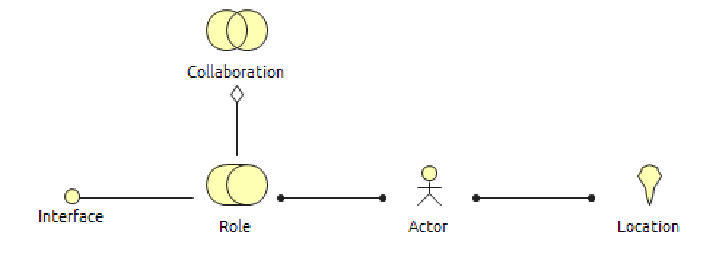
\includegraphics[width=13cm,height=6cm]{arquitectura/negocio/imgs/m_organizacion}
	\caption{Modelo de Organización}{\scriptsize \textbf{Fuente:} Archimate 2.0 \cite{WEB7}}
\end{figure}


\subsubsection{Caso}

En la organización que se presenta dentro de las propiedades horizontales se puede ver roles muy bien definidos.

%%grafo
\begin{figure}[th!]
	\centering
	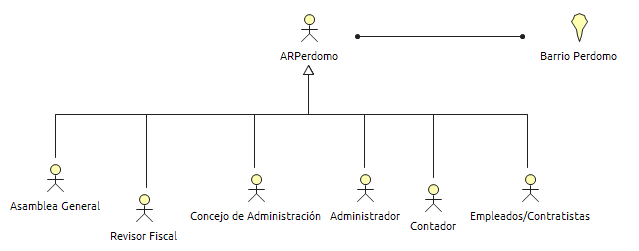
\includegraphics[width=12cm,height=6cm]{arquitectura/negocio/imgs/organizacion}
	\caption{Caso de Organización}{\scriptsize \textbf{Fuente:} Imagen propia}
\end{figure}


\subsubsection{Punto de Vista de Función de Negocio}

La función de negocio permite determinar las tareas que debe realizar cada rol

%%grafo

\begin{figure}[th!]
	\centering
	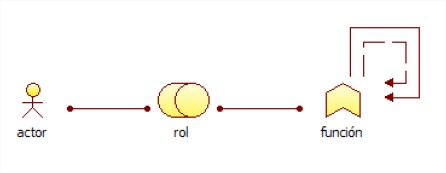
\includegraphics[width=7cm,height=4cm]{arquitectura/negocio/imgs/funcion-negocio}
	\caption{Modelo de Función de negocio}{\scriptsize \textbf{Fuente:} Archimate 2.0 \cite{WEB7}}
\end{figure}

\subsubsection{Caso}

En el punto de vista presentado a continuación se reflejan las funciones de cada rol, especificando las labores que de cada uno de ellos.

%%grafo
\begin{figure}[th!]
	\centering
	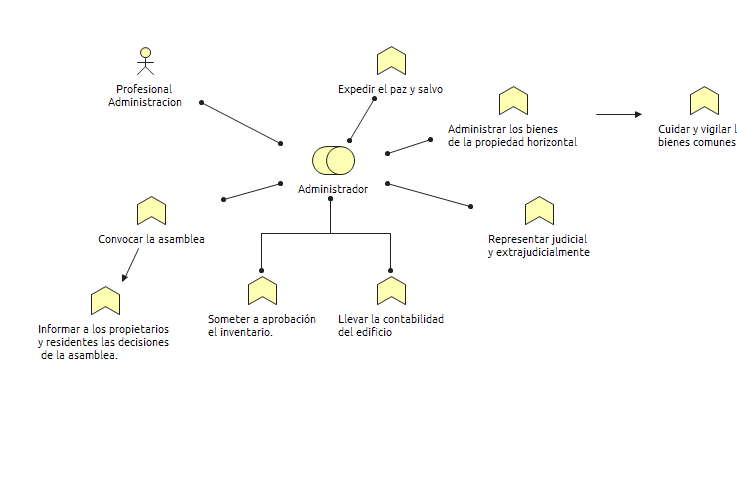
\includegraphics[width=16cm,height=9cm]{arquitectura/negocio/imgs/funciones-1}
	\caption{Funciones administrador}{\scriptsize \textbf{Fuente:} Imagen propia}
\end{figure}

\begin{figure}[th!]
	\centering
	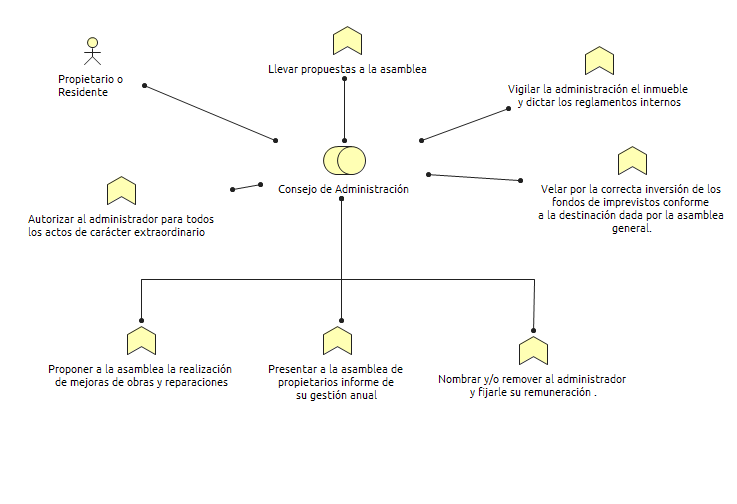
\includegraphics[width=15cm,height=9cm]{arquitectura/negocio/imgs/funciones-2}
	\caption{Funciones consejo administrativo}{\scriptsize \textbf{Fuente:} Imagen propia}
\end{figure}


\begin{figure}[th!]
	\centering
	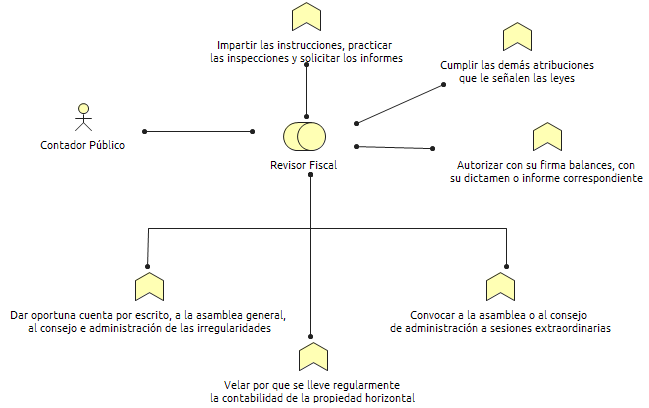
\includegraphics[width=15cm,height=9cm]{arquitectura/negocio/imgs/funciones-3}
	\caption{Funciones revisor fiscal}{\scriptsize \textbf{Fuente:} Imagen propia}
\end{figure}

\newpage

\subsubsection{Punto de Vista de Proceso de Negocio}

Cada proceso de negocios constituye un esfuerzo por mejorar las operaciones y las funciones de la compañía. 

%%grafo

\begin{figure}[th!]
	\centering
	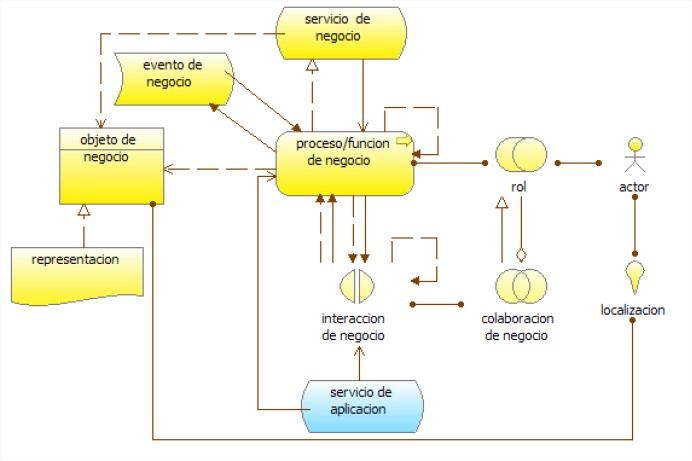
\includegraphics[width=11cm,height=6cm]{arquitectura/negocio/imgs/proceso-negocio}
	\caption{Modelo de Proceso de negocio}{\scriptsize \textbf{Fuente:} Archimate 2.0 \cite{WEB7}}
\end{figure}

\subsubsection{Caso}

En el punto de vista de proceso de negocio, se presenta el Core de la organización por medio del proceso fundamental que da vida a la empresa.

%%grafo
\begin{figure}[th!]
	\centering
	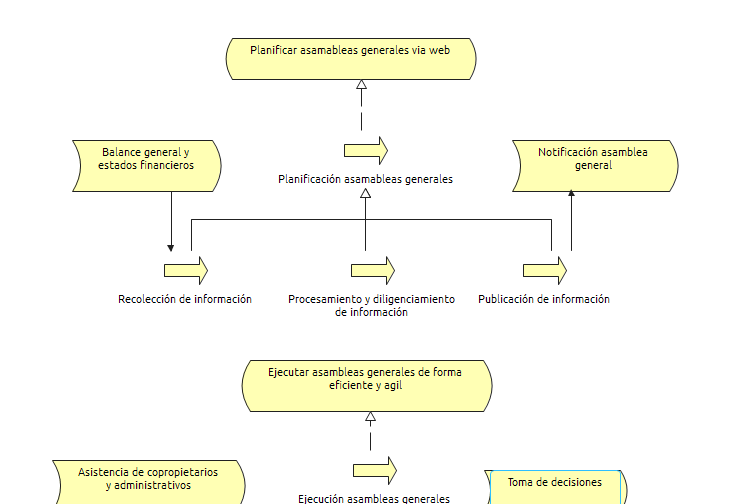
\includegraphics[width=15cm,height=7cm]{arquitectura/negocio/imgs/proceso}
	\caption{Proceso de negocio}{\scriptsize \textbf{Fuente:} Imagen propia}
\end{figure}
\newpage

\subsubsection{Punto de Vista de Cooperación de Proceso de Negocio}

La cooperación dentro del proceso de negocio permite reflejar los difetentes componentes que interactuan dentro del proceso.

%%grafo

\begin{figure}[th!]
	\centering
	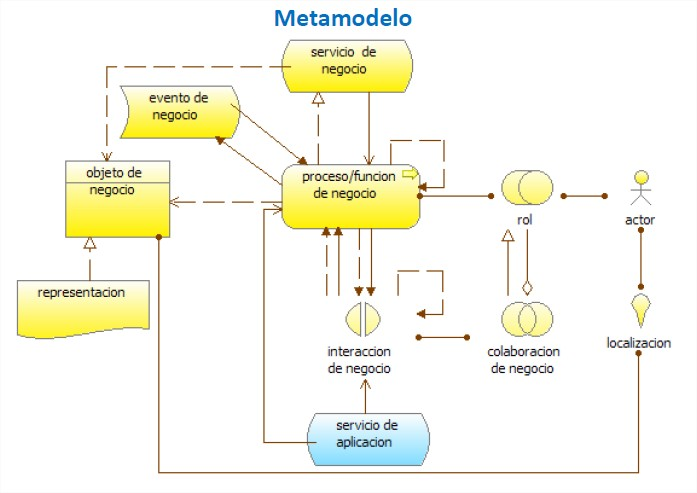
\includegraphics[width=12cm,height=6cm]{arquitectura/negocio/imgs/Coop-proceso-negocio}
	\caption{Modelo de Cooperación proceso de negocio}{\scriptsize \textbf{Fuente:} Archimate 2.0 \cite{WEB7}}
\end{figure}

\subsubsection{Caso}

En el siguiente diagrama se representan las diferentes colaboraciones que se tienen en el proceso de la planificación de las asambleas generales de copropiedad horizontal.

%%grafo
\begin{figure}[th!]
	\centering
	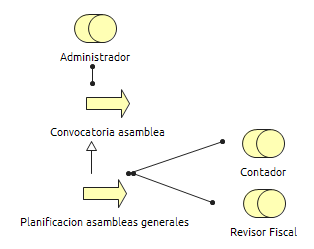
\includegraphics[width=12cm,height=7cm]{arquitectura/negocio/imgs/cooperacion-proceso}
	\caption{Cooperación de proceso de negocio}{\scriptsize \textbf{Fuente:} Imagen propia}
\end{figure}
\newpage

\subsubsection{Punto de Vista de Producto}

El punto de vista de producto permite ver la interacción dle producto final con el cliente.

%%grafo

\begin{figure}[th!]
	\centering
	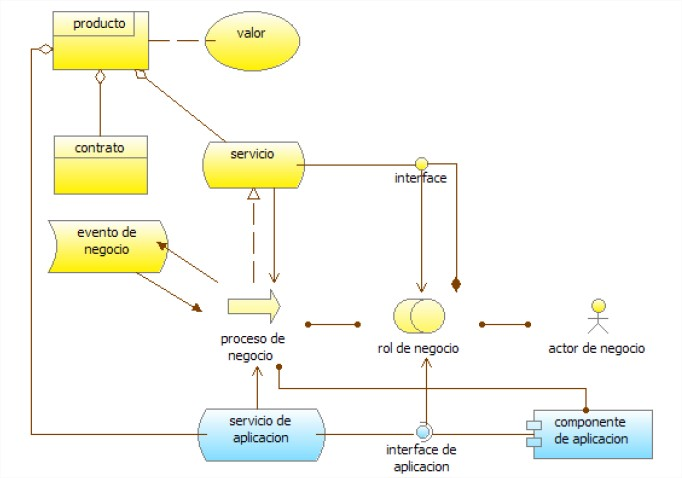
\includegraphics[width=12cm,height=6cm]{arquitectura/negocio/imgs/producto.jpg}
	\caption{Modelo de Producto}{\scriptsize \textbf{Fuente:} Archimate 2.0 \cite{WEB7}}
\end{figure}

\subsubsection{Caso}

Para el caso del desarrollo de asambleas generales se presenta el producto y su interacción con el cliente, que pára el caso son el Administrador, el copropietario, etc.

%%grafo
\begin{figure}[th!]
	\centering
	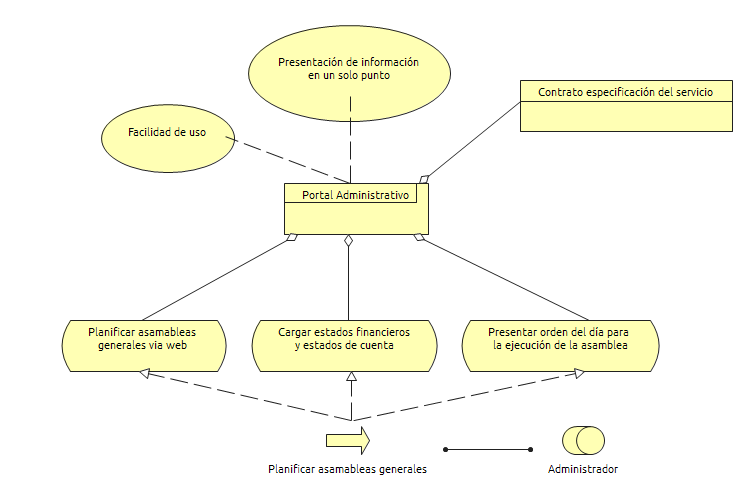
\includegraphics[width=12cm,height=7cm]{arquitectura/negocio/imgs/producto.png}
	\caption{Producto de negocio}{\scriptsize \textbf{Fuente:} Imagen propia}
\end{figure}
\newpage